\chapter{Centrado}

Es una de las etapas del procesamiento de im�genes. Recibe como par�metro de entrada no solo la imagen si no un rango de color previamente seleccionado.
Todos los p�xeles cuyo color est� dentro de este rango, formaran un conjunto. El conjunto de las coordenadas cartesianas de estos p�xeles dentro de la imagen.
Vamos a llamar centro de masas (c. m.), a la media de las coordenadas de todos los p�xeles que forman el conjunto, de esta manera el centro de masas ser� la coordenada de un p�xel que puede o no pertenecer al conjunto, pero que representa el centro de la mayor concentraci�n de elementos de este. La coordenada x ser� la media aritm�tica de todas las coordenadas x de este conjunto y lo mismo con la y.
$ X = \dfrac{\Sigma x_{i}}{k} $ , desde i=1..k, siendo k el cardinal del conjunto y \forall x_{i} \epsilon conjunto.
$ Y = \dfrac{\Sigma y_{i}}{k} $ , desde i=1..k, siendo k el cardinal del conjunto y \forall y_{i} \epsilon conjunto.

El objetivo es centrar el centro de masas dentro de la imagen. As� estaremos centrando la regi�n de inter�s. El centrado implica un desplazamiento de todos los p�xeles de la imagen.
 
Ejemplo:
\begin{center}
\begin{tabular}{|c|c|}
\hline 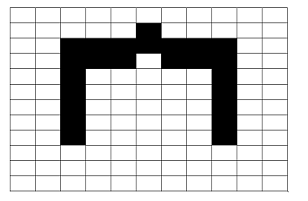
\includegraphics[scale=1]{centrado.png}  & 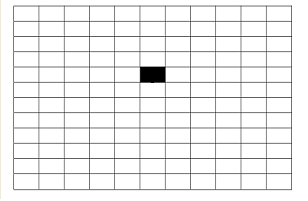
\includegraphics[scale=1]{centrado2.png}  \\ 
\hline 
\end{tabular} 
La imagen de la izquierda muestra una imagen en blanco y negro. El color elegido es el negro.
La imagen de la derecha muestra cual ser�a la coordenada que representa el centro de masas del conjunto de p�xeles negros.
\end{center} 

Seg�n esto, los p�xeles que cumplen la propiedad de estar dentro del rango del color elegido son:
{(6,2),(3,3),(4,3),(5,3),(6,3),(7,3),(8,3),(9,3), (3,4),(4,4),(5,4),(6,4),(7,4),(8,4),(9,4),(3,5),(3,6),(3,7),(3,8),(3,9),(9,5),(9,6),(9,7),(9,8),(9,9)}
y por tanto el c. m. cae en la posici�n (6, 4.84) \cong (6,5)
siendo el centro de la imagen la posici�n (6,6)

La posici�n del c. m. no esta en el centro de la imagen. La distancia que hay que desplazar la imagen es el modulo entre el punto central de la imagen y el punto del centro de masas. Por tanto movemos todos los p�xeles de la imagen n posiciones verticalmente y m posiciones horizontalmente para cuadrar el c. m. con el centro de la imagen. En este proceso hay p�xeles de la imagen original que se pierden y otros que se crean y no tienen un valor concreto, estos ser�n creados con el color del entorno, ya que se supone que no son de inter�s.
Bas�ndonos en el ejemplo anterior, el centro de masas esta desplazado respecto al centro de la imagen una posici�n hacia arriba, por lo que hay que desplazar todos los p�xeles de la imagen una posici�n hacia abajo. Esto destruye la fila de abajo y crea una fila nueva en la parte superior a cuyos p�xeles se les asignara el color blanco.

\begin{center}
\begin{tabular}{|c|c|}
\hline 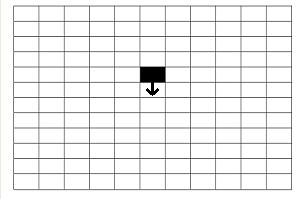
\includegraphics[scale=1]{centrado3.png}  & 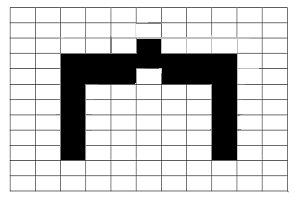
\includegraphics[scale=1]{centrado4.png}  \\ 
\hline 
\end{tabular} 
La imagen de la izquierda muestra la direcci�n en que se deben desplazar todos los p�xeles.
La imagen de la derecha muestra el resultado del desplazamiento.
\end{center} 

Ejemplo real
\begin{center}
\begin{tabular}{|c|c|}
\hline \includegraphics[scale=1]{regiones.png}  & \includegraphics[scale=1]{filtrado.png}  \\ 
\hline 
\end{tabular} 
\end{center} 

\section{Curiosidad}
El centrado tiene otra utilidad. Debido a que necesita hacer el calculo de cuantos p�xeles cumplen la propiedad de estar dentro del rango de color, si resulta que no hay en toda la imagen ninguno que la cumpla, el m�todo no devuelve la imagen centrada, si no que devuelve NULL. Tal y como esta implementado el pipeline si un modulo saca como estructura de datos un puntero a NULL, las siguientes operaciones que se realizar�an sobre esta estructura dejan de hacerse, esto aumenta la velocidad del programa si no hay gestos o carteles frente al robot, ya que disminuye en gran cantidad el numero de instrucciones realizadas. Se podr�a decir que el centrado es un detector de objetos de inter�s que mantiene al pipeline en \textit{stand by} mientras que no se detecten objetos frente a la c�mara.

